\chapter{导论}

\section{准备工作}

\href{https://www.stata.com/}{Stata} 是一款商业统计软件,你可以从 Stata 公司购买获得。最新版的 Stata 是 Stata 15.1,支持中界面文:

\begin{figure}[htbp]
  \centering
  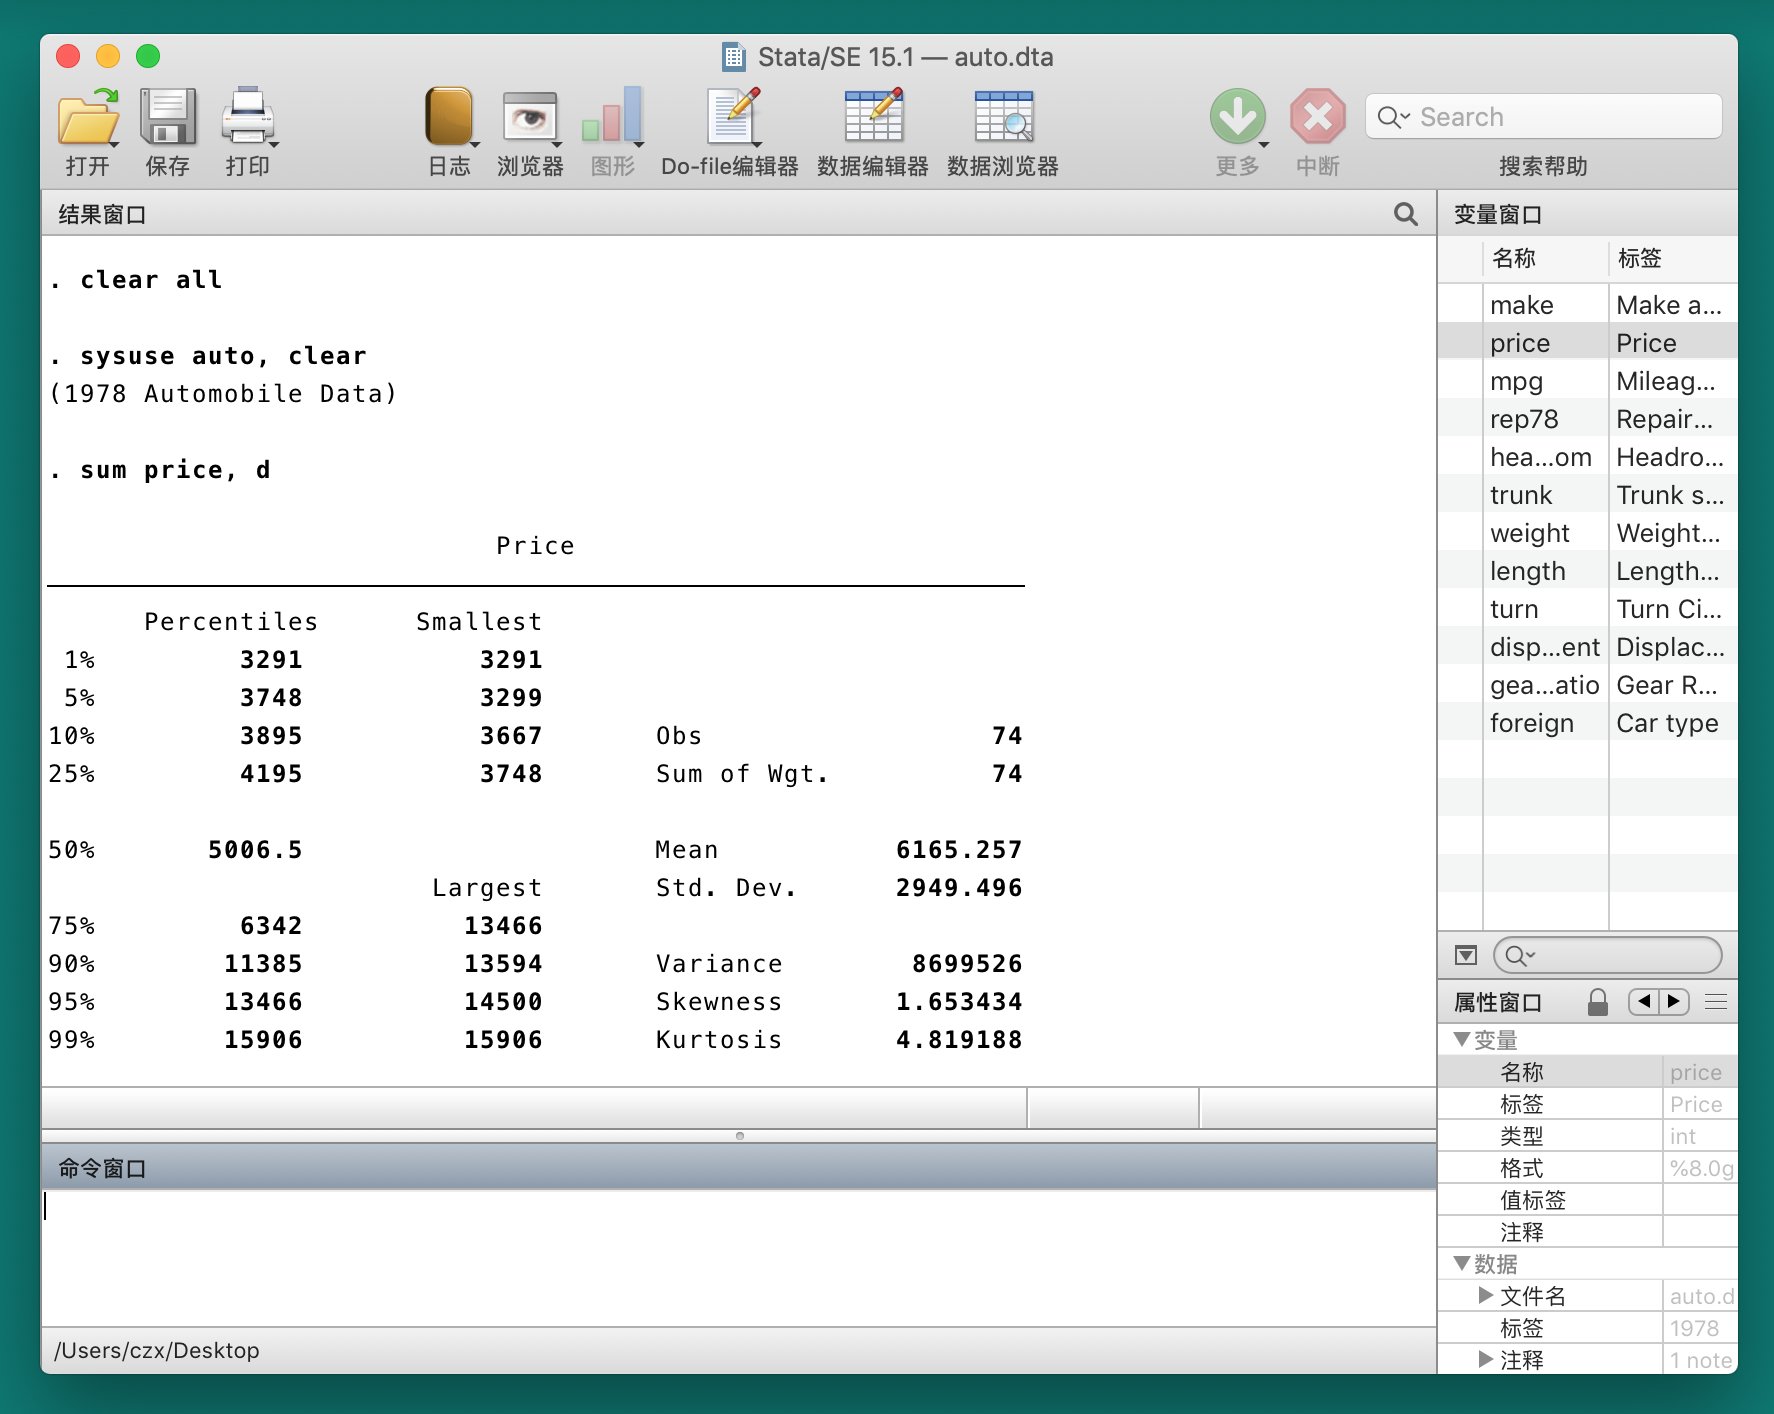
\includegraphics[width = \textwidth]{assets/stataui.png}
  \caption{Stata 15.1 for Mac 的界面}
  \label{fig:stataui}
\end{figure}

目前为止,你需要知道Stata最直接的使用方法是从命令窗口输入代码,然后回车运行,结果会显示在结果窗口。

如果你需要写很多行代码,这种使用方式就不是一个好习惯了,为了研究的可重复性,你最好建立一个 do 文件,然后将你的代码一行行输入在 do 文档里保存:

\begin{figure}[htbp]
  \centering
  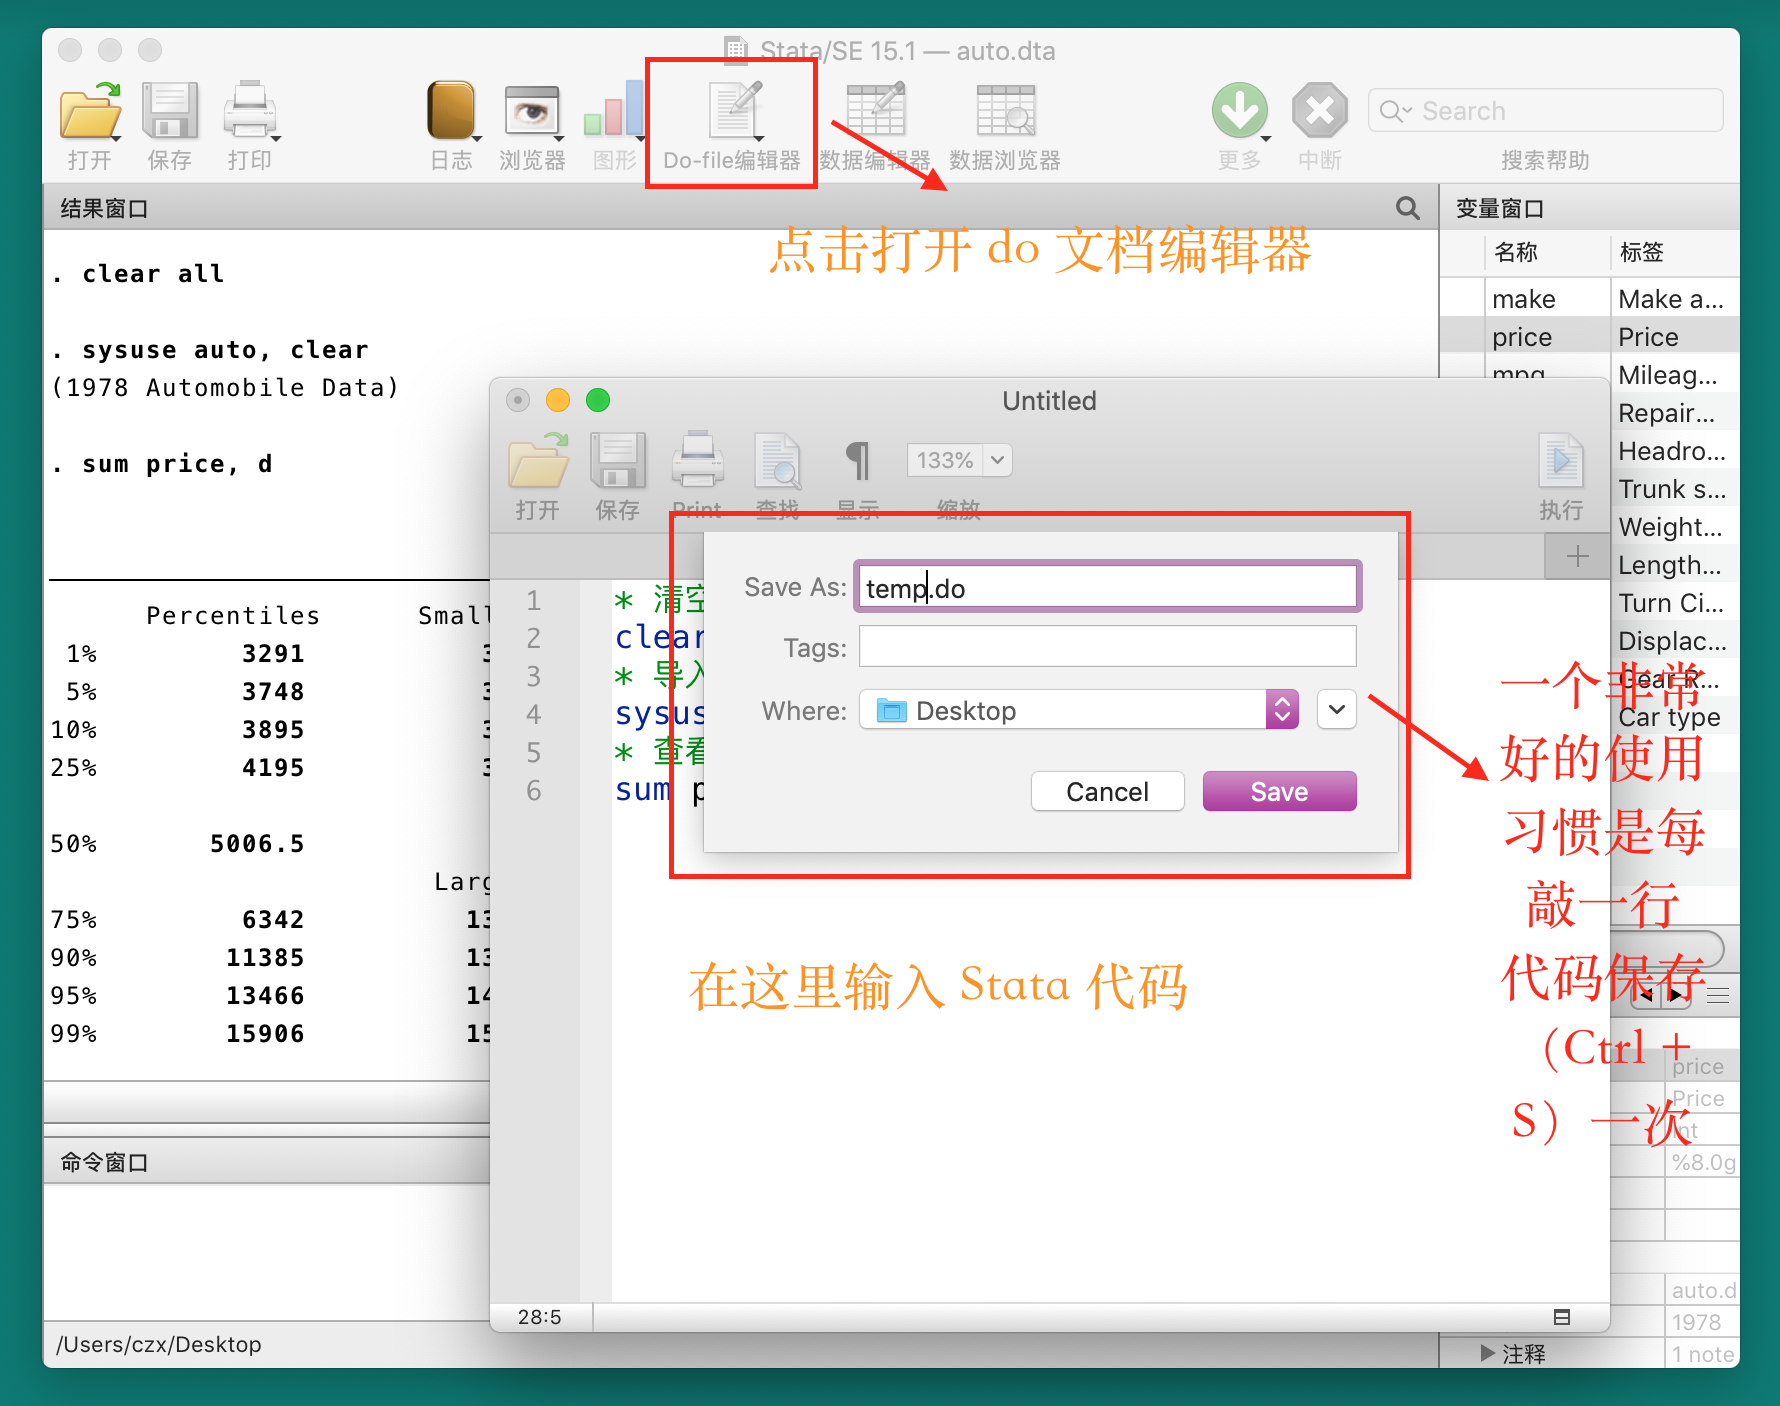
\includegraphics[width = \textwidth]{assets/do-file.png}
  \caption{Stata15.1 for Mac 的 do 文档编辑器界面}
  \label{fig:dofile}
\end{figure}

事实上,Stata 自带的这个编辑器并不好用,为了提高敲代码的效率,建议使用 Sublime Text3 编辑器。具体配置方法可以参考我的网站文章 \href{https://www.czxa.top/posts/59313/}{Stata安装与Sublime Text3配置教程}。

\begin{figure}[htbp]
  \centering
  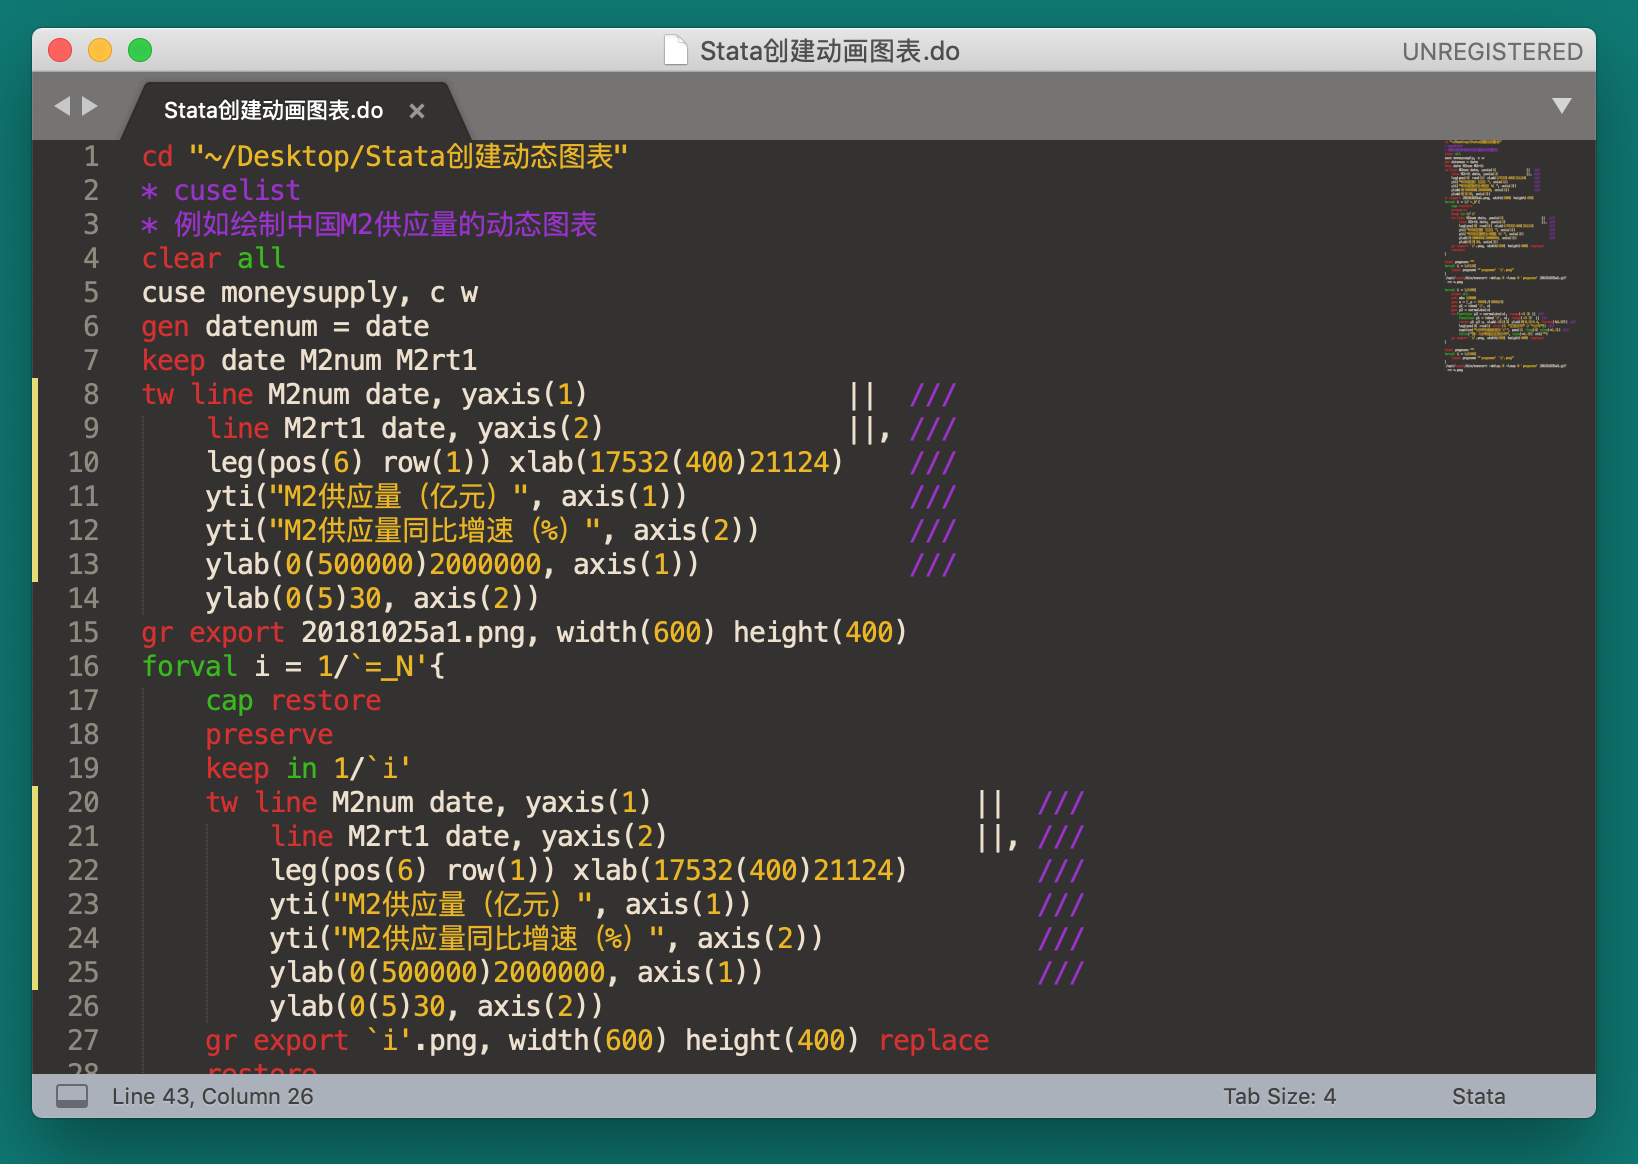
\includegraphics[width = \textwidth]{assets/sublime.png}
  \caption{Sublime Text3 for Mac 界面}
  \label{fig:sublime}
\end{figure}

你还可以从 \href{https://github.com/andrewheiss/SublimeStataEnhanced}{SublimeStataEnhanced} 获取最新的配置方法。

\section{stata4ds 命令包}

为了更方便的讲述,我开发了一个命令包,这个命令包涵盖了本书所需要的所有数据集和部分外部命令。你可以运行下面的 Stata 命令进行安装。

\begin{lstlisting}
  * 首先需要安装 github 命令,这个命令可以用来安装 GitHub 上的 Stata 命令。
  net install github, from("https://haghish.github.io/github/")
  * 然后使用 github 命令安装 stata4ds
  github install stata4ds, replace
\end{lstlisting}

除此之外,你还需要安装以下外部命令:

\begin{lstlisting}
  * 安装 cuse 命令包
  github install czxa/cuse, replace
  * 安装 finance 命令包
  github install czxa/finance, replace
  * 安装 tidy 命令包
  ssc install tidy, replace
  * 安装 superscatter 命令
  net install superscatter, from(http://digital.cgdev.org/doc/stata/MO/Misc) replace
  ...未完待续...
\end{lstlisting}

\begin{remark}
  实际上在安装 stata4ds 命令包的最后这些命令会被自动逐一地安装。
\end{remark}

\section{运行 Stata 代码}

前面一节展示了一段 Stata 代码的运行结果,在本书中的代码是像这样的:

\begin{lstlisting}
  display 1 + 2
  *> 3
\end{lstlisting}

而你运行上面的代码之后,结果窗口显示的结果应该是这样的:

\begin{lstlisting}
  . display 1 + 2
  3
\end{lstlisting}

\section{获取帮助}

Stata 提供了非常详细完善的帮助文档,要查阅帮助文档,你可以使用 \textcolor{third3}{help} 命令,例如查看 \textcolor{third3}{clear} 的帮助文档:

\begin{lstlisting}
help clear
\end{lstlisting}

\begin{figure}[htbp]
  \centering
  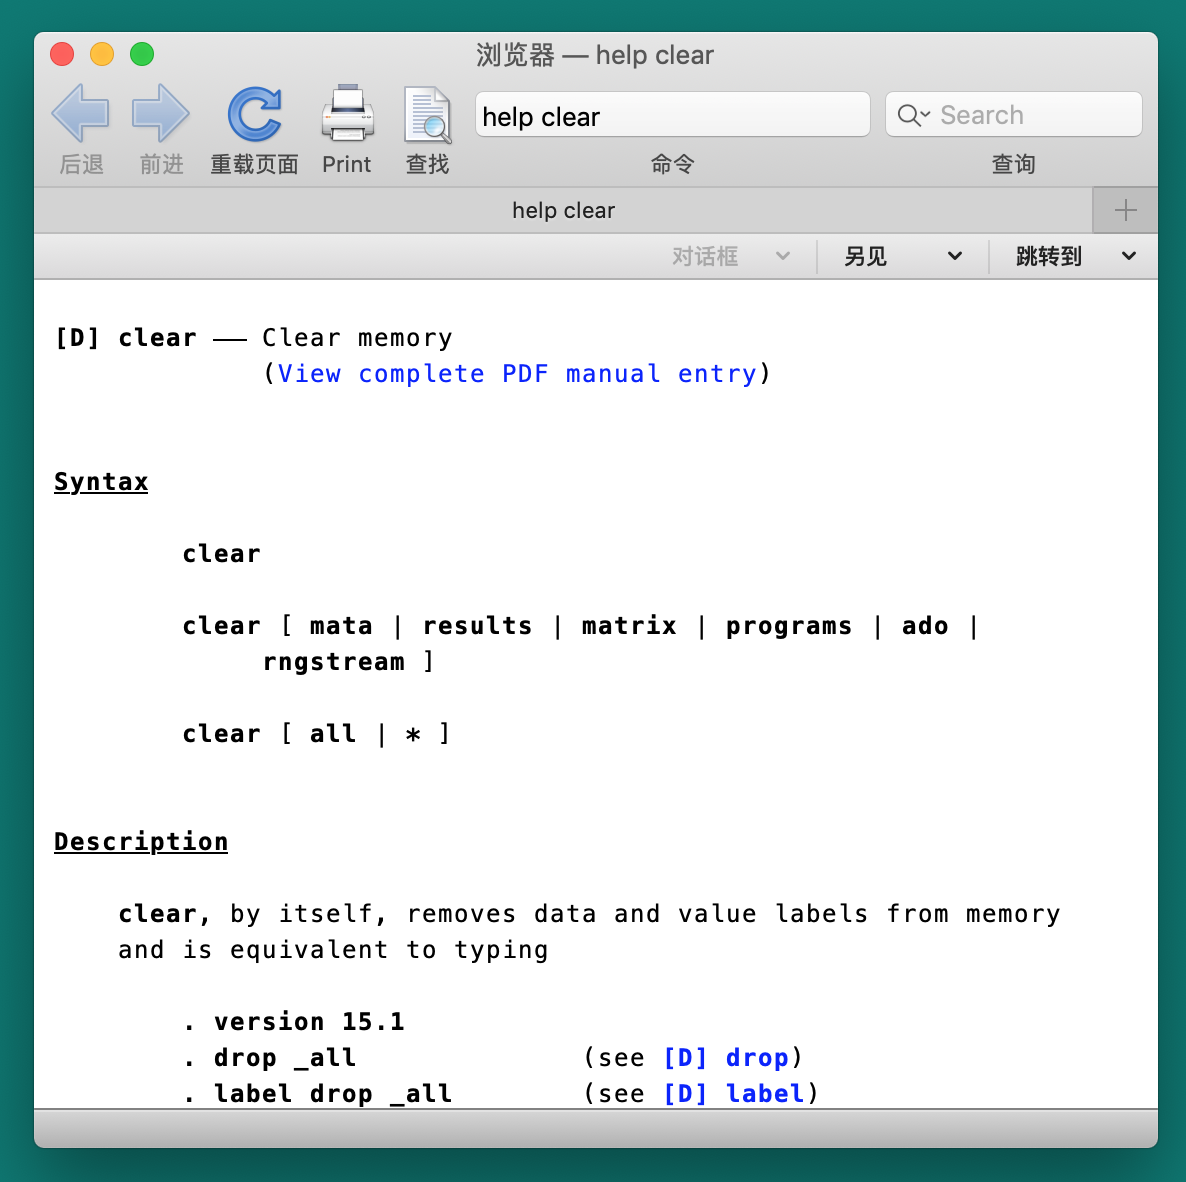
\includegraphics[width = 0.6\textwidth]{assets/clear.png}
  \caption{clear 命令的帮助文档}
  \label{fig:clear}
\end{figure}

Stata 还拥有着丰富的网络资源,你可以使用 \textcolor{third3}{search} 和 \textcolor{third3}{findit} 命令搜索,例如我想查找 \textcolor{third3}{egen} 相关的内容:

\begin{lstlisting}
  search egen
  findit egen
\end{lstlisting}

Stata 官网上也有着丰富的 Stata 资源。此外,Stata15 比起前代的 Stata 有巨大的进步,如果你想了解 Stata15 的新功能,可以到 Stata 的官网查看:\href{https://www.stata.com/new-in-stata/}{New in Stata 15}。

\begin{figure}[htbp]
  \centering 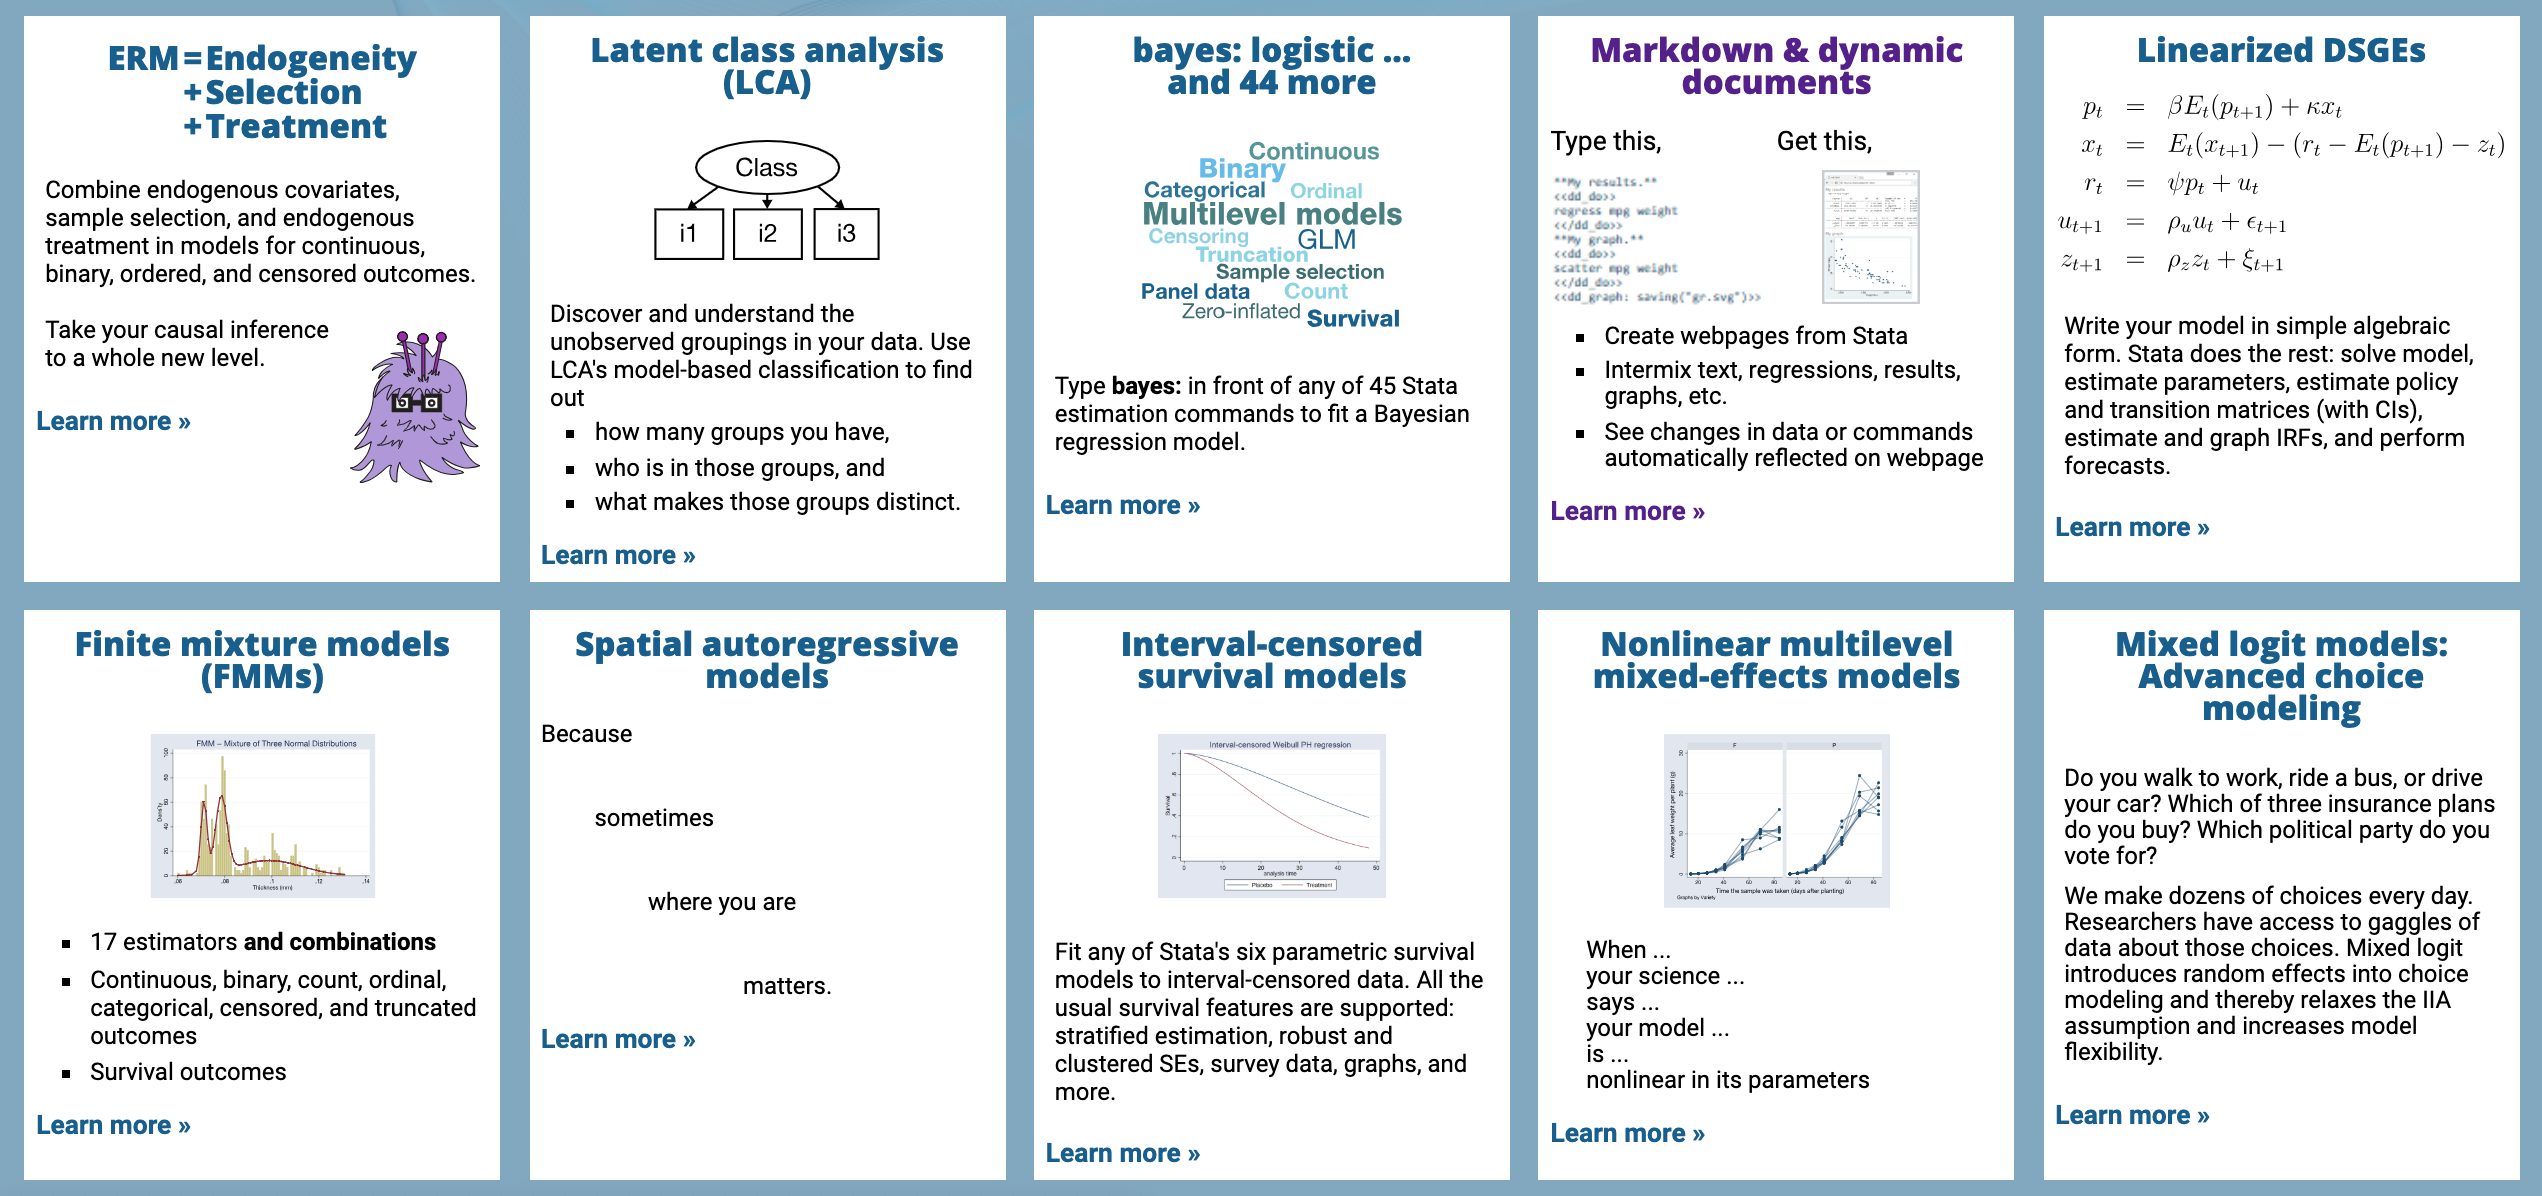
\includegraphics[width= 0.8\textwidth]{assets/newinstata15.png}
  \caption{Stata15 的新功能}
  \label{fig:newinstata15}
\end{figure}

你还可以在 \href{https://www.statalist.org/forums/}{Stata List} 和 \href{https://blog.stata.com/}{Stata Blog} 获取 Stata 使用的资源和帮助。另外, \href{https://github.com/topics/stata}{GitHub \# Topic: stata} 上也有一些非常好用的 Stata 命令和学习资源。

下一章实际上并不是本书想要编排进来的内容,而是作者之前在担任计量经济学助教的时候编写的讲义,虽然比较粗略(毕竟讲义这种东西的目的只是帮助演讲者组织思路)。但是我相信通过下一章内容的学习,你将能够更轻松的进行本书的学习。因此特意将该讲义插入进来(其实只是想凑字数)。
